\chapter{State of the Art}
\label{chap:state_of_the_art}

The objective of this section is to review current regulatory frameworks, hardware and software components, and advanced security schemes relevant to NFC-based access control.


\section{NFC Frameworks and Standards}

This section reviews the principal ISO/IEC standards that govern contactless cards interoperability, security and form factor. We examine ISO/IEC 14443 \cite{ref23} for proximity communication protocols, ISO/IEC 7816-4 \cite{ref24} for APDU-based command structures and ISO/IEC 7810 \cite{ref25} for physical card dimensions.

\subsection{Contactless personal identification: ISO/IEC 14443}

ISO/IEC 14443 \cite{ref23} is the international standard that defines how contactless identification devices (e.g., smart cards, RFID key fobs or NFC readers) should communicate at close range (up to about 10 cm) with reader stations.

It is structured in four complementary blocks that cover from the physical characteristics of the cards to the data exchange protocols and the mechanisms for managing multiple transponders simultaneously. An overview of each of these four components is presented below \cite{ref65}:

\begin{itemize}
	\item \textbf{Part 1: Physical Characteristics.} Establishes the physical specifications of proximity cards, such as their size and format (ISO/IEC 7810 ID-1). It ensures that devices comply with a common physical standard, which is essential for hardware compatibility between different implementations.
	
	\item \textbf{Part 2: Signaling and transmission.} Defines the modulation and coding parameters of the signal. In Type A mode, ASK (Amplitude Shift Keying) modulation at 13.56 MHz with Manchester coding is used. In Type B mode, ASK-BPSK (Binary Phase Shift Keying) is used to avoid collisions. These schemes guarantee the robustness of wireless communication.
	
	\item \textbf{Part 3: Initialization and anti-collision.} Introduces the card detection and selection process. The anti-collision technique allows the identification of multiple cards within the reading field by assigning unique identifiers (UIDs). This feature is essential in environments where multiple cards may be present simultaneously.
	
	\item \textbf{Part 4: Transmission Protocol.} Details the exchange of commands and data between the card and the reader. It supports a transmission structure based on data blocks, where commands such as authentication, read, write and encryption are handled. This is critical in security applications, where a secure exchange of information is required.
\end{itemize}

Compliance with ISO/IEC 14443 ensures that both NFC chips and readers (e.g., NTAG424 DNA and PN532) operate under a standard and optimized protocol. The following aspects are key:

\begin{itemize}
	\item \textbf{Interoperability:} it allows the integration of different devices that follow the same standard, reducing compatibility issues between hardware and access control software \cite{ref66}.
	
	\item \textbf{Security:} The standard supports authentication and encryption mechanisms at the protocol level, which is essential for protecting data in sensitive applications such as access control. In combination with algorithms such as AES-128 implemented in the NTAG424 DNA chips, the system can perform secure and encrypted authentication \cite{ref67}.
	
	\item \textbf{Transmission efficiency:} The modular transmission structure ensures that data is exchanged quickly and reliably while maintaining low latency, which is crucial in real-time access systems.
\end{itemize}

\subsection{Identification cards communication: ISO/IEC 7816-4}

ISO/IEC 7816-4 \cite{ref24} establishes the common language and the structure of the messages (APDUs) that allow a reader and a card to exchange instructions and data in an orderly and secure manner. This standard is key in applications that require authentication and secure transmission, such as NFC access control.

In this context, ISO/IEC 7816-4 specifies key technical aspects that enable these functionalities, including the use of APDU structures, system response management and transmission control protocols. These elements are described below to understand how they contribute to secure system operation \cite{ref68}:

\begin{itemize}
	\item \textbf{APDU (Application Protocol Data Unit):} APDUs are the basis of communication between card and reader, divided into two types:
	\begin{itemize}
		\item \textit{Command APDU:} Contains the command, with a header consisting of the CLA (instruction class), INS (instruction), P1 and P2 (parameters) fields, together with the data and the Le (expected length of response) field.
		\item \textit{Response APDU:} Returns the requested data and the SW1 SW2 status code.
	\end{itemize}
	
	\item \textbf{Application Selection:} The SELECT command allows you to choose an application on the card based on its AID (Application Identifier), making it easy to interact with cards that manage multiple applications.
	
	\item \textbf{File Management:} The card manages structured data files, with READ, WRITE and UPDATE commands. These commands allow secure control of stored information.
	
	\item \textbf{Authentication and Encryption:} ISO/IEC 7816-4 supports authentication and encryption mechanisms through the use of keys, facilitating the implementation of AES or DES to secure communications.
\end{itemize}

In the NFC access control system, ISO/IEC 7816-4 enables secure transmission using APDUs, which support credential management and two-factor authentication. NTAG424 DNA chips, with AES-128 encryption capability, can be efficiently integrated using this standard to ensure that the exchanged data is protected and structured correctly.

\subsection{Contactless cards: ISO/IEC 7810}

ISO/IEC 7810 \cite{ref25} defines the physical dimensions and general characteristics of identification cards, including NFC cards used in access control systems. This standard establishes specifications for the manufacture of ID cards in several standard formats, the most common being:

\begin{itemize}
	\item \textbf{ID-1 format:} 85.60 mm × 53.98 mm dimensions, typical of credit and debit cards.
	\item \textbf{ID-2 format:} 105 mm × 74 mm, like passport size.
	\item \textbf{ID-3 format:} 125 mm × 88 mm, used in passports and other travel documents.
	\item \textbf{ID-000 format:} 25 mm × 15 mm, smaller size format used in SIM cards.
\end{itemize}

Each format specifies a thickness of 0.76 mm \cite{ref25}, providing consistency in the cards for handling and reading in devices. These standards enable interoperability in systems that require user identification and verification, ensuring that cards fit into readers and access control devices in a uniform manner.

ISO/IEC 7810 is especially relevant for identification and authentication applications, such as NFC-based access control systems. Standardized dimensions and physical properties ensure that cards remain uniform, which facilitates their integration into NFC devices and card readers. In addition, this standard allows the card design to be rugged and durable, withstanding repeated use in access control environments.


\section{NFC Read/Write Libraries and Modules}
\label{sec:nfc_libs}


The following section reviews advanced NFC security schemes and their practical applications. In recent years, NFC technology has transcended its original use as a means of proximity reading to become the basis for multi-level security architectures. By combining cryptographic elements, challenge-response protocols and additional authentication factors, it is possible to ensure both data confidentiality and communication integrity. In addition, the integration of NFC with IoT platforms and cloud services enables dynamic and remote management of access to facilities \cite{ref69}.

Before getting into advanced schemes, it is useful to understand the most common starting point for NFC access control applications: authentication by unique UID reading. This method simply consists of matching the unique identifier engraved on the chip with an authorized list on the server; its main virtue is simplicity, as it does not require complex cryptographic protocols or additional key exchange. However, since it is based exclusively on a static value that can be easily captured and duplicated, it lacks protection mechanisms against cloning or replay attacks.

These limitations are particularly evident when using cards such as MIFARE Classic, whose security has been widely compromised \cite{ref70} (see section 3.2.1). It is therefore necessary to contrast these ``basic'' systems with solutions that incorporate encryption, mutual authentication and other dynamic security factors.


\section{NFC secure access control systems}

The following section reviews advanced NFC security schemes and their practical applications. In recent years, NFC technology has transcended its original use as a means of proximity reading to become the basis for multi-level security architectures. By combining cryptographic elements, challenge-response protocols and additional authentication factors, it is possible to ensure both data confidentiality and communication integrity. In addition, the integration of NFC with IoT platforms and cloud services enables dynamic and remote management of access to facilities \cite{ref69}.

Before getting into advanced schemes, it is useful to understand the most common starting point for NFC access control applications: authentication by unique UID reading. This method simply consists of matching the unique identifier engraved on the chip with an authorized list on the server; its main virtue is simplicity, as it does not require complex cryptographic protocols or additional key exchange. However, since it is based exclusively on a static value that can be easily captured and duplicated, it lacks protection mechanisms against cloning or replay attacks.

These limitations are particularly evident when using cards such as MIFARE Classic, whose security has been widely compromised \cite{ref70} (see section 3.2.1). It is therefore necessary to contrast these ``basic'' systems with solutions that incorporate encryption, mutual authentication and other dynamic security factors.

\subsection{NFC Cards and PIN}

One robust security solution commonly offered related to the NFC technology is its combination with PIN authentication. Pins are short passwords, usually formed by numbers (although they may contain another type of characters), they are usually four to six characters long. On the one hand, PINS are easy to remember by humans. On the other hand, they are easy to guess or hack. In order to try to mitigate this, they usually have some kind of restriction regarding the number of tries an user has before being locked out \cite{ref30}.

The combination of these two technologies is based on the concept of multifactor authentication, users authenticate using something they have (NFC card) and something they know (PIN). There are two approaches in the usage of PIN in this type of system, using the same PIN for every user or using one for each user.

Leading companies like HID global offer several hardware solutions like the HID® multiCLASS SE® RK40 \cite{ref75}, figure~\ref{fig:hid_multiclass}, that is one single module including an NFC reader and a keypad.

\begin{figure}[h!]
	\centering
	\includegraphics[width=0.6\textwidth]{imaxes/pin.png} 
	\caption{HID® multiCLASS SE® RK40 NFC PIN Reader, HID ICLASS SE card and tag}
	\label{fig:hid_multiclass}
\end{figure}

\subsection{NFC with Biometrics}

Biometrics are personal authenticators related to a physical human trait that can unequivocally identify a person. It should be permanent, measurable in a quick and easy way, and fast to compare against stored information.

The convergence of NFC technology with biometric authentication systems has given rise to advanced security and usability solutions in various fields. It is widely used in access control systems, secure payment methods and smartphone authentication \cite{ref83}. This integration allows the identification and verification of users in an efficient and secure manner, taking advantage of the benefits of both technologies. It is also based on the concept of multifactor authentication, where users authenticate using something they have (NFC card) and something they are (biometric).

Biometrics popularity is due to its lack of change during time, the most used biometric is the fingerprint, unique pattern of whorls and lines on the fingertips of a person. For centuries, it has been a reliable method of identifying people; from a crime record to a passport. Also, fingerprint readers use four different technologies: optical, which records an image; capacitance, ultrasonic and thermal, which identify and map ridges \cite{ref30}. There are also other biometrics that can be used but not to the same extent that are: hand geometry, iris, retina, face and voice.

\subsection{Enhanced Version 2 (EV2) NFC Mutual Authentication protocol}

Enhanced Version 2 (EV2) \cite{ref29} is NXP’s latest mutual-authentication scheme for NFC cards, built on ISO/IEC 14443-4 framing and AES-128 CMAC. EV2 ensures that both reader (PCD) and card (PICC) prove knowledge of a shared secret and derive fresh session keys on each transaction, protecting against replay, cloning and man-in-the-middle attacks.

Mutual authentication using AES-128 is a common practice in various industries that require secure communications and protection against unauthorized access. One of the most secure protocols in the access control industry which uses mutual authentication and AES-128 is SEOS \cite{ref31}, developed by HID and has its own SEOS cards. Which consists of an AES-128 encryption key for protecting data confidentiality and a MAC key that guarantees message integrity by means of authentication codes.

The EV2 exchange adheres to ISO/IEC 14443-4 command structure:
\begin{itemize}
	\item The card is selected and detected, in which the reader is aware of the card and sends it a WAKE-UP command, which is responded with its corresponding ATQA (Answer to Request).
	\item The communication is established using the commands RATS (Request for Answer to Select) and ATS (Answer to Select).
	\item The reader sends an AES-128 encrypted challenge to the card. The card decrypts and responds with another encrypted challenge. If both challenges are successful, a secure channel is established.
	\item APDU (Application Protocol Data Units) commands are sent to read credentials inside the Seos™ Vault, the card returns the encrypted data, ensuring its integrity by means of the MAC key.
\end{itemize}

In addition to SEOS, NXP’s broader MIFARE family, NTAG 424 DNA and DESFire EV2/EV3 \cite{ref32}, implements EV2 mutual authentication to different ends. NTAG 424 DNA’s EV2 protocol is trusted by vendors like RFID.it, Shenzhen Focused Smartech Co., Seritag, and ZipNFC \cite{ref84}; it follows the EV2 flow described above and activates CMAC-based confidentiality and integrity once the challenge–response succeeds (Figure~\ref{fig:ntag424_ev2}). MIFARE DESFire EV2/EV3 offers a comparable process but introduces variations in session-key handling and secure-messaging (IV + SM) to meet diverse application requirements.

\begin{figure}[h!]
	\centering
	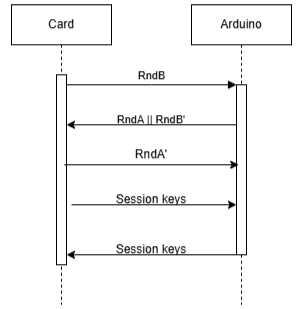
\includegraphics[width=0.7\textwidth]{imaxes/MA_diagram.png} % Cambia el nombre por tu imagen real
	\caption{NTAG424 mutual authentication diagram, random nonces and session keys exchange}
	\label{fig:ntag424_ev2}
\end{figure}

\subsection{NFC with Internet Of Things}

The Internet of Things (IoT) refers to a network of interconnected physical devices like sensors, actuators and embedded systems that communicate and exchange data over the Internet to enable intelligent automation and monitoring. The use of NFC, combined with the IoT, has enabled the development of advanced access control and management systems. These systems offer enhanced security, real-time traceability and greater automation compared to traditional methods based on static credentials. The combination of these technologies takes advantage of leverage short-range wireless communication capabilities to improve connectivity, interaction and management of IoT devices \cite{ref33}.

These systems are capable of implementing authentication and access control in secure infrastructures, managing assets in real-time, remotely monitoring through cloud platforms and automating processes without human intervention \cite{ref34}.

The most typical architecture of these types of systems is based on ESP32, which allows communication via the internet. Also, several devices can be part of these systems with different functionalities, the most remarkable in the access control field are:
\begin{itemize}
	\item Cameras: they use ESP32 to communicate
	\item Locks: they use ESP32 to communicate
	\item Smart Sensors: Devices that monitor environmental variables such as movement, and can communicate via NFC to turn on the lights.
\end{itemize}

There are several companies implementing these technologies such as Bosch Security and Safety Systems, which offer advanced access control solutions that integrate NFC and IoT technology. Its systems enable centralized access management in real time, using NFC-enabled mobile devices to authenticate users and control entrances to facilities. It is also interesting to mention Honeywell International, that has developed access control systems that incorporate NFC and IoT to provide secure authentication and efficient access management in corporate and industrial environments.

\subsection{NFC with Cloud}

Cloud services are remote computing resources such as storage, processing power and software applications hosted on distributed servers and accessed over the Internet. The combination of NFC and cloud services has boosted the development of advanced solutions for access management, authentication and user traceability. These systems allow data to be stored and processed on cloud servers, eliminating dependence on local storage and facilitating real-time access from any device with an Internet connection. In addition, they offer scalability, redundancy and advanced security through data encryption and multi-layered authentication \cite{ref35}.

There are some projects which can be used as examples of the different ways of implementing this technology. A cloud-based attendance management system that uses NFC cards to record employee check-in and check-out, reducing human error and increasing operational efficiency \cite{ref36}. These systems usually use TLS to communicate with the webserver, in this case, it sends the information with the UID of the NFC tag and records the hour the employee attended to the facilities in the webserver. Also, there are other projects that are similar \cite{ref37} that use the same function but in this case it uses the arduino database and a web server programmed in php which stores name, date and id. These resources can be hosted on AWS, Google Cloud or Microsoft Azure, which offer a higher level of scalability and security.

\subsection{NFC with Locks}

In the field of access control systems, there are various electronic lock technologies that differ according to their operating mechanisms, installation requirements and operating and maintenance costs. High-security mechanical locks, based on cylinders and latches reinforced with high-strength alloys, offer great robustness against physical attacks but are incompatible with centralized credential management solutions and have high maintenance costs. Electromechanical locks—such as electric frame locks or recessed solenoids—allow integration with card or code control systems by introducing a motorized actuator but have high power consumption and reduce their effectiveness after a certain number of mechanical cycles \cite{ref38}.

Stand-alone electronic locks, or ``smart locks'', incorporate microcontrollers, RFID or Bluetooth readers and internal batteries, which facilitate access management via smartphones, wireless networks or digital credentials, at the cost of a higher unit cost and a complexity of configuration and security that, if not properly managed, can introduce new vulnerabilities. Compared to these alternatives, magnetic locks stand out for their simplicity of construction, their durability and their ability to be integrated into large-scale infrastructures. These devices consist of an electromagnet rigidly fixed to the door frame and a ferromagnetic plate installed in the door leaf; when tension is applied, a holding force is generated that can exceed 600 kg, guaranteeing resistance to forced opening attempts.

With no moving parts, magnetic locks minimize mechanical wear and maintenance costs, and by operating in ``fail-safe'' mode, releasing the door when the power fails, they naturally meet evacuation requirements in emergency situations requiring immediate release of exits. In addition, their installation requires only two conductors and one signal contact, which simplifies wiring standardization and favors their adoption at multiple control points (gates, turnstiles, barriers), maintaining operational consistency and facilitating centralized management \cite{ref39}. Also, these types of locks allow the usage of REX (request-to-exit) devices, which release the door control mechanisms and facilitate safe egress.

\subsubsection{REX (request-to-exit)}

A Request-to-Exit (REX) sensor is an access control device that guarantees the free opening of an exit door fitted with an electric magnetic lock, without the need to enter credentials, by detecting the proximity of a person using infrared, microwave or laser scanning technologies; when activated, it sends a signal to deactivate the electromagnet and allow immediate passage. Equivalently, many installations use push buttons or panic bars mounted on the door leaf: their simple mechanical actuation interrupts the power supply to the maglock, releasing it instantly and ensuring both rapid evacuation and compliance with safety and accessibility regulations. Solutions such as ASSA ABLOY's Aperio systems \cite{ref40} or Bosch Security Systems' security doors \cite{ref41} often integrate REX sensors and push-button or panic bar optics interchangeably, adapting to the operational and compliance needs of each environment.


\section{NFC cards}

This section presents the main families of NFC cards used in identification and access control applications, with special emphasis on their technical characteristics, storage capacities and security mechanisms.

Although there are multiple manufacturers of NFC-compatible chips and cards, the market for secure identification solutions is largely dominated by NXP Semiconductors \cite{ref80}. It develops the most widely used NFC cards, including MIFARE, DESFire, NTAG and SmartMX. Also, there are other companies such as Infineon Technologies, which offer secure NFC tags too, such as the OPTIGA Authenticate and secure memory chips \cite{ref82}.

In this section, MIFARE Classic is exposed due to its importance in the early stages of this technology, which then leads to the evolution into other cards that support cryptographic operation for increased security, such as NTAG424.

\subsection{MIFARE Classic and similar NFC cards}

MIFARE Classic \cite{ref28}, figure~\ref{fig:mifare_classic} \cite{ref81}, is a model of NFC card that was introduced as a cost-effective and widely compatible solution, operating in the 13.56 MHz band and based on the ISO/IEC 14443-A standard. These cards offer limited storage capacity, designed primarily for simple applications such as public transportation, basic access and small payments. They were pioneers in identification systems, enabling popularization of the use of NFC. Also, due to their low cost and simplicity, they were massively implemented in environments with basic security needs.

MIFARE Classic are vulnerable to cloning attacks due to their Crypto1 encryption scheme, considered weak by current standards \cite{ref70}. These vulnerabilities have limited their use in applications requiring high levels of security. The model of cards is gradually being replaced by more secure technologies such as MIFARE DESFire or NTAG 413 DNA, which implement advanced encryption such as AES \cite{ref71}. However, widespread deployment and cost constraints mean that many organizations still rely on these insecure cards, delaying a full migration to more robust alternatives.

\begin{figure}[h!]
	\centering
	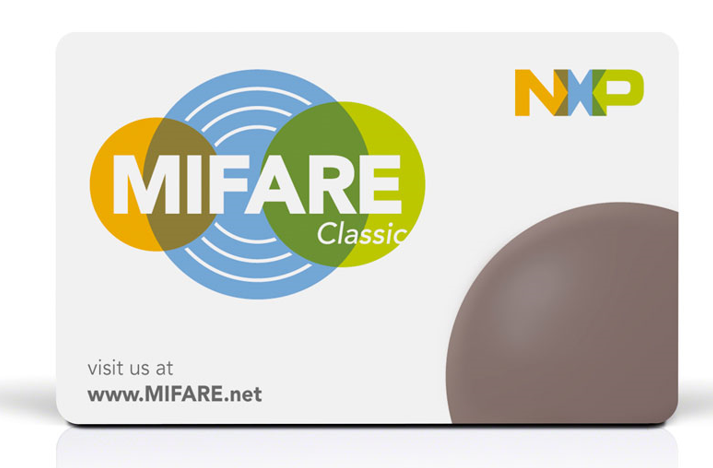
\includegraphics[width=0.4\textwidth]{imaxes/mifare1.png} % Cambia el nombre por tu imagen real
	\caption{MIFARE Classic card}
	\label{fig:mifare_classic}
\end{figure}

\subsection{NTAG 424 DNA}

With the growing demand for security, new solutions in the NFC card field have emerged, such as the NTAG 424 DNA \cite{ref29} cards, developed by NXP Semiconductors, which offer significant improvements over their predecessors. This card incorporates the AES-128 encryption standard, providing stronger protection against cloning attempts and unauthorized access. Also, they integrate SUN (Secure Unique NFC) Authentication technology, which allows the generation of unique and secure messages in each interaction, ensuring the authenticity of the communication and preventing replay attacks. Importantly, NTAG 424 DNA fully supports the Enhanced Version 2 (EV2) mutual-authentication protocol, allowing them to establish secure channels with NFC readers.

NTAG 424 DNA is able to generate unique and random identifiers for each transaction, enhancing user privacy and preventing unauthorized tracking. In addition, they are designed to be fully compatible with standard NFC devices, facilitating their integration into mobile applications and modern systems. Last but not least, one of the key features of this card is its communication speed, which can be highlighted in faster data transfer rates and improving efficiency in operations that require real-time information exchange.

\subsection{Key Management with NTAG424}

The NTAG 424 DNA card integrates a robust cryptographic key management system designed to ensure secure and flexible access control and data protection. This system is based on key hierarchy and diversification, allowing for the generation of unique keys per tag and application, while maintaining compatibility with shared functionalities when necessary.

As described in Section 8.2.4 of the official NXP datasheet \cite{ref42}, the card supports a key diversification mechanism using a Master Personalization Key (or Master Secret) that is securely stored and managed in the backend infrastructure. This master key is used only during initialization or key regeneration processes to derive diversified keys.

The NTAG 424 DNA supports five distinct 128-bit AES keys, each with specific roles in the authentication and access control structure:

\begin{itemize}
	\item \textbf{AppKey0}: Used for mutual authentication Enhanced version 2 (EV2) standard, as seen in figure~\ref{fig:ntag424_ev2} \cite{ref42}, and read access to NDEF (NFC Data Exchange Format) files.
	\item \textbf{AppKey1}: Enables writing to NDEF files and allows verification of data integrity via CMACs.
	\item \textbf{AppKey2}: Grants access to proprietary data files that may contain sensitive or application-specific information.
	\item \textbf{AppKey3}: Controls access to advanced security features, such as SDM (Secure Dynamic Messaging), which allows protected reading of encrypted and integrity-checked data.
	\item \textbf{AppKey4}: Reserved for extended functionalities and future implementations.
\end{itemize}

Each key slot supports a Key Version Byte (1 byte) that identifies the current version of the key, enabling efficient management and update of credentials. This feature is particularly useful in systems where key rotation or renewal is a security requirement. Moreover, the tag allows for key updating and configuration through authenticated sessions using the ChangeKey and ChangeKeySettings commands. These operations can only be performed after a successful mutual authentication, ensuring that key management remains secure and protected against unauthorized access.

This architecture provides a balance between security, scalability, and flexibility, making the NTAG 424 DNA suitable for a wide range of secure NFC applications, including access control, secure identification, and ticketing systems.

\begin{figure}[h!]
	\centering
	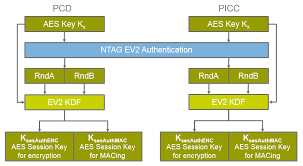
\includegraphics[width=0.7\textwidth]{imaxes/EV2ntag.png} % Cambia el nombre por tu imagen real
	\caption{NTAG EV2 Authentication using AES-128 encryption: on the left PCD (reader) and on the right PICC (NTAG)}
	\label{fig:ntag424_ev2}
\end{figure}
